\section{Method}
\subsection{Problem Formulation}

We consider embodied policy learning from visual observations and language instructions. Let $o$ denote the current observation, $l$ denote the task instruction, and $a_{1:H}$ denote an action chunk of horizon $H$. A standard visuomotor policy models the conditional distribution
\begin{equation}
    p(a_{1:H} \mid o, l),
\end{equation}
which directly maps the current perceptual context to a sequence of actions. World Action Models (WAMs) augment this formulation by introducing future visual observations as an intermediate variable. Let $v_{1:T}$ denote future visual observations over a prediction horizon $T$. Many existing WAMs follow an \emph{imagine-then-execute} factorization:
\begin{equation}
    p(a_{1:H} \mid o, l)
    =
    \int p(v_{1:T} \mid o, l)\,
    p(a_{1:H} \mid o, l, v_{1:T})\, dv_{1:T},
\end{equation}
where the model first predicts future observations and then conditions action generation on the imagined future. In practice, this is typically implemented either by jointly denoising future video and actions within a shared model, or by first generating future video and then feeding it to an inverse dynamics or action prediction module. Some prior WAMs further wrap this formulation in an outer auto-regressive rollout, which we omit here for simplicity and controlled comparison.

Our starting point is the observation that the effectiveness of WAMs may arise from two distinct factors: \emph{(i)} the video prediction objective used during training, which can encourage the model to learn physically meaningful latent representations, and \emph{(ii)} explicit future generation during inference, which may provide additional foresight for action prediction. Existing WAM formulations usually couple these two factors, since the same model both learns from future video prediction and explicitly synthesizes future observations at test time. We design Fast-WAM to decouple these two factors. During training, it retains world modeling as a co-training signal; during inference, however, it does not explicitly generate future observations. Instead, Fast-WAM predicts actions directly from the current observation and instruction,
\begin{equation}
    p_\theta(a_{1:H} \mid o, l),
\end{equation}
while using latent world representations shaped by video co-training. In this sense, Fast-WAM has a direct-policy interface at test time, similar to standard VLA policies, while its representation learning remains grounded in WAM-style video modeling during training. Formally, let $z(o, l)$ denote the latent world representation produced by the video backbone conditioned on the current context. Fast-WAM uses this representation to parameterize the action distribution,
\begin{equation}
    p_\theta(a_{1:H} \mid o, l)
    =
    p_\theta(a_{1:H} \mid z(o, l)).
\end{equation}
The key difference from imagine-then-execute WAMs is that $z(o, l)$ is obtained by a single forward encoding pass, rather than by explicitly sampling or denoising future observations $v_{1:T}$ at inference time.

\subsection{Model Architecture}

\paragraph{Overview.}
Fast-WAM is designed to preserve the training benefits of world modeling while removing the inference cost of explicit future imagination. During training, it jointly learns action prediction and video modeling, encouraging the visual backbone to capture physically meaningful motion and interaction structure. During inference, Fast-WAM does not explicitly generate future observations. Instead, it keeps only the clean latent tokens of the first observation frame, processes them with the video model in a single forward pass, and uses the resulting latent world representation for direct action generation. This gives Fast-WAM a direct-policy interface at test time while retaining WAM-style video supervision during training.


\paragraph{Architecture.}
Fast-WAM is built on top of the video Diffusion Transformer (DiT) from Wan2.2-5B~\cite{wan2025}, which serves as the world modeling backbone. We also reuse its pretrained text encoder and video VAE: task language is encoded by the built-in T5 encoder and provided to all tokens through cross-attention, while visual observations are mapped into latent video tokens by the pretrained VAE. On top of this backbone, we introduce an action expert DiT for action chunk generation. The full model is organized as a Mixture-of-Transformer (MoT) architecture with shared attention between the video and action branches, as illustrated in Figure~\ref{fig:model_arch}.

We organize the input tokens into three groups: clean latent tokens of the first observation frame, which serve as the shared visual anchor; noisy latent tokens of future video frames, which are used only during training for video modeling; and action tokens, which are processed by the action expert for action generation. All token groups attend to the language embeddings through cross-attention. A structured attention mask controls the information flow between these groups. During training, future noisy video tokens attend bidirectionally within the video branch and can access the clean first-frame tokens; action tokens attend bidirectionally within the action branch and can also access the clean first-frame tokens. Crucially, action tokens cannot attend to future video tokens, and the clean first-frame tokens do not attend to any other tokens. This ensures that both video modeling and action prediction are grounded in the same visual context while preventing future information from leaking into the action branch. We provide the full training and inference masks in Figure~\ref{fig:mask}.

At inference time, Fast-WAM removes the future video branch entirely: only the clean first-frame latent tokens are retained and passed through the video backbone once to produce latent world features for the action expert. Since no future noisy video tokens are instantiated and no explicit future video denoising is performed, Fast-WAM incurs substantially lower inference cost than standard imagine-then-execute WAMs.

\begin{figure}[t]
    \centering
    \begin{subfigure}[t]{0.6\linewidth}
        \centering
        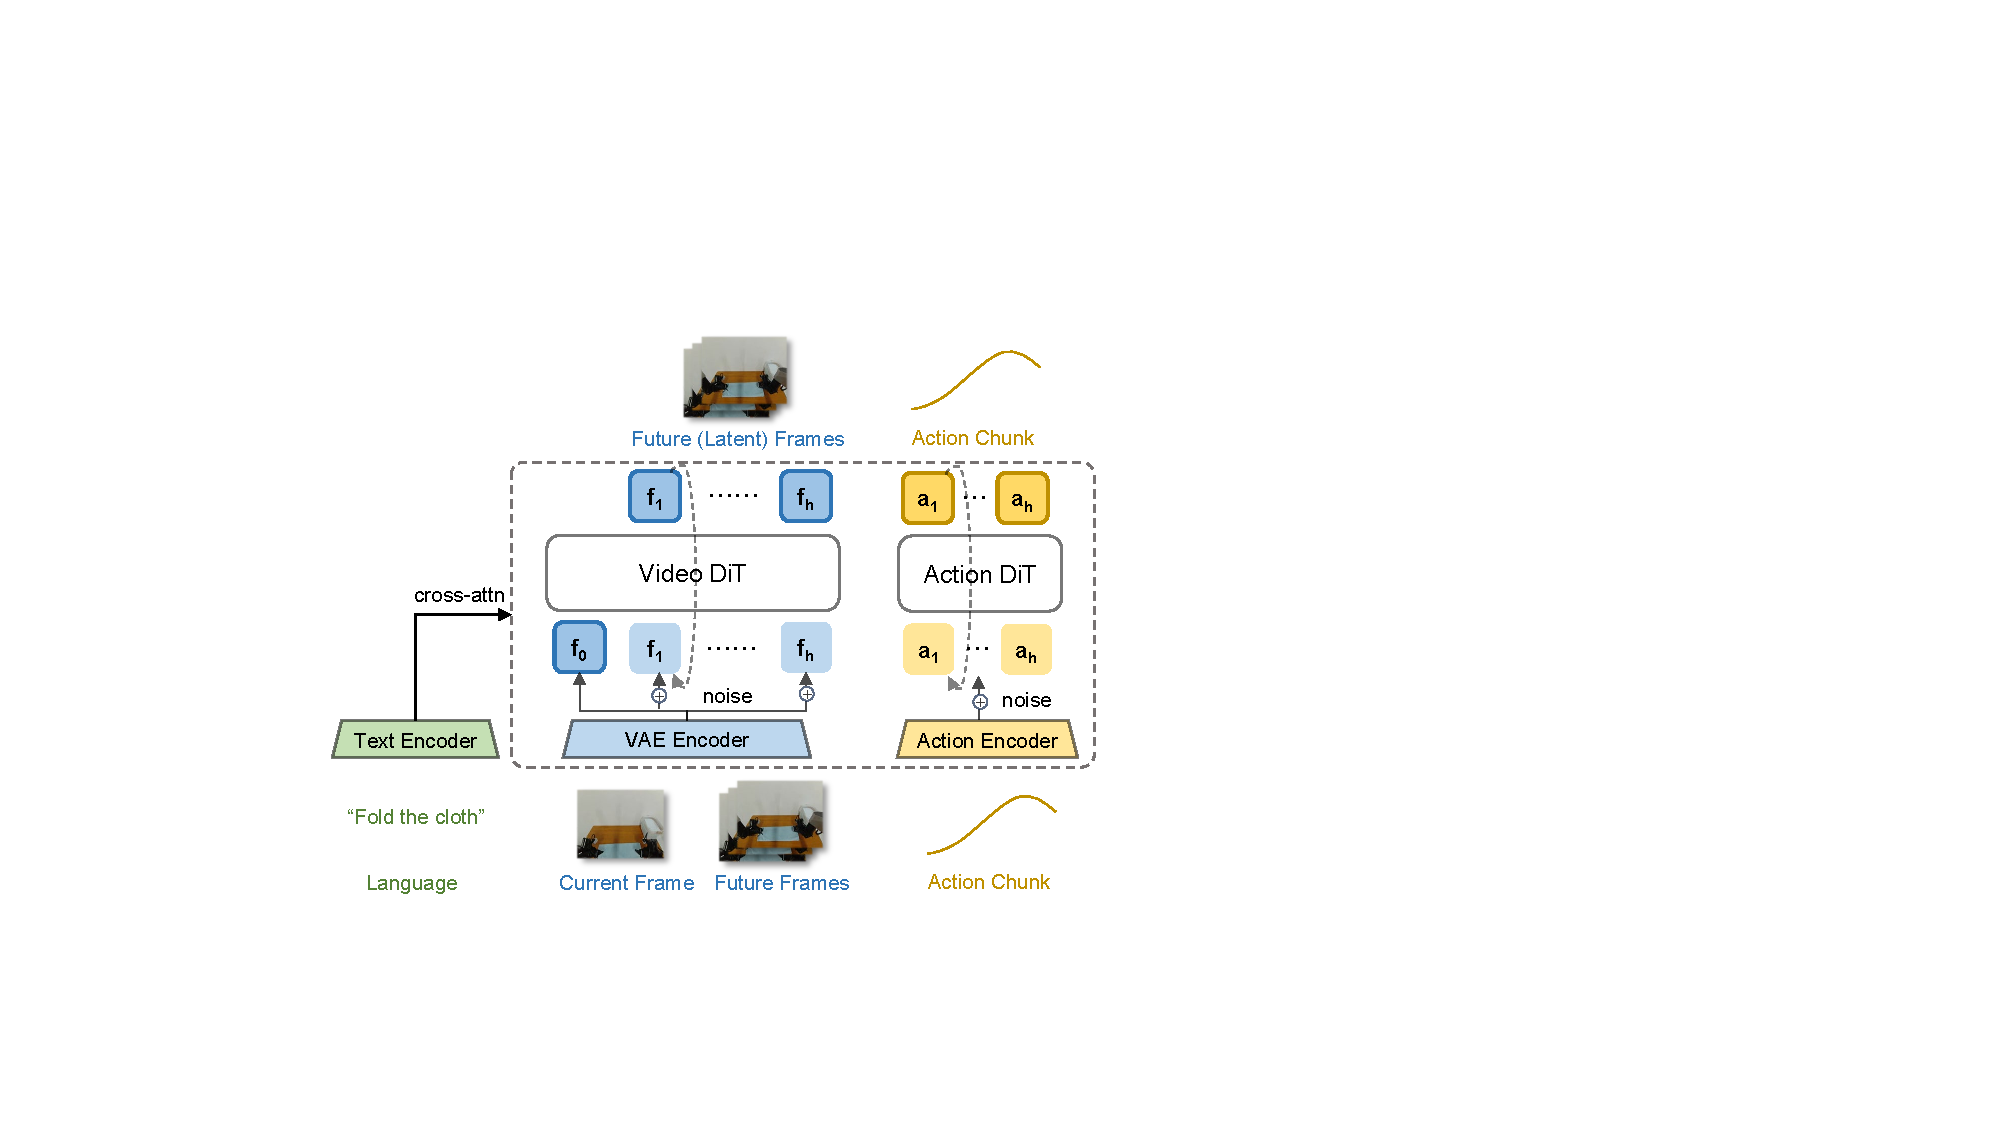
\includegraphics[width=\linewidth]{figs/model_arch.pdf}
        \caption{Fast-WAM model architecture.}
        \label{fig:model_arch}
    \end{subfigure}
    \hspace{0.05\linewidth}
    \begin{subfigure}[t]{0.2\linewidth}
        \centering
        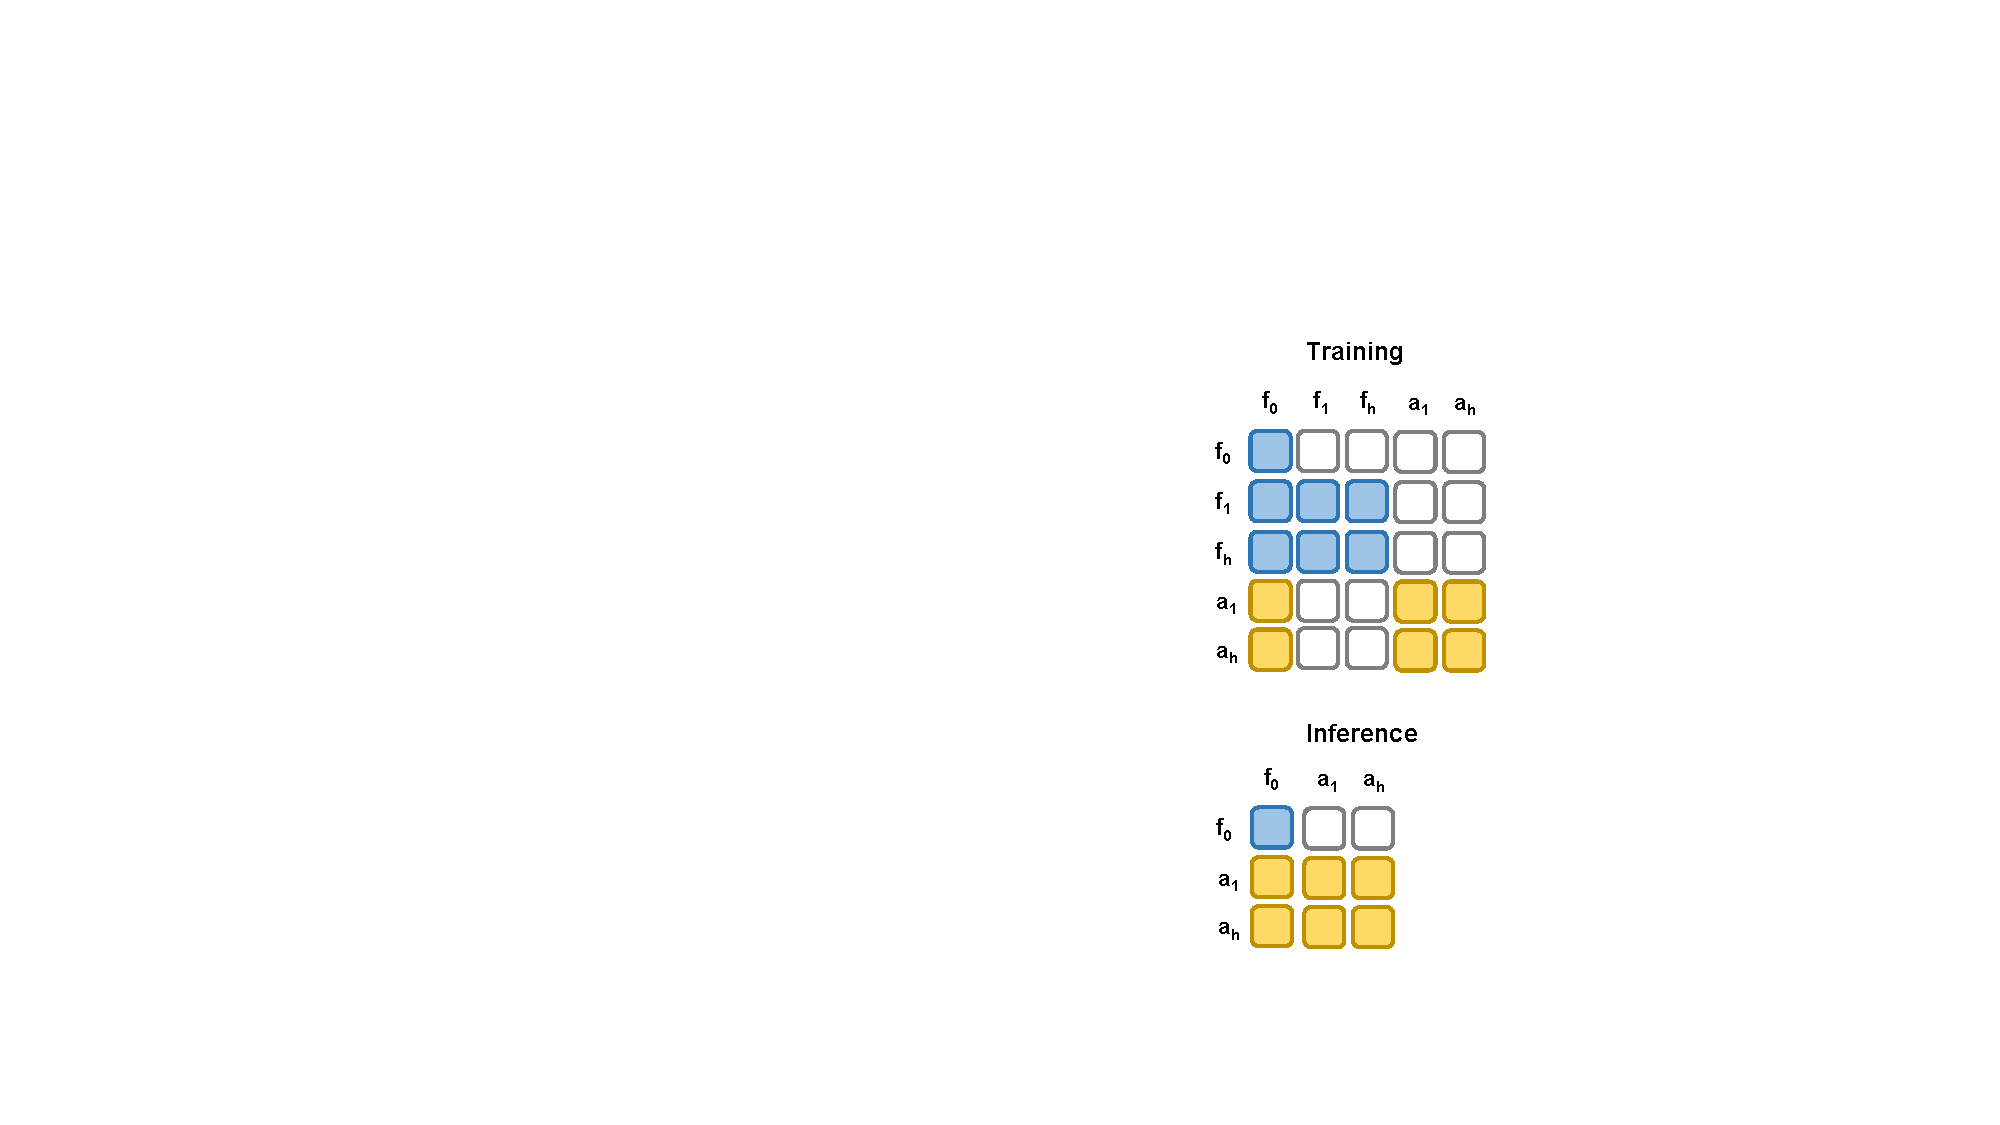
\includegraphics[width=\linewidth]{figs/mask.pdf}
        \caption{Training and inference masks.}
        \label{fig:mask}
    \end{subfigure}
    \caption{Fast-WAM architecture and the structured attention mask used to disentangle video co-training from action generation.}
    \label{fig:fastwa_arch}
\end{figure}

\paragraph{Training objective.}
Fast-WAM is trained with a joint flow matching objective over action tokens and future video latents. Given a target variable $y$ (either an action chunk $a_{1:H}$ or future video latents $z_{1:T}$), we sample Gaussian noise $\epsilon \sim \mathcal{N}(0, I)$ and a time step $t \in(0,1)$, and construct the interpolated sample
\begin{equation}
    y_t = (1-t)\, y + t\, \epsilon.
\end{equation}
The model is trained to predict the corresponding velocity field with a standard flow matching objective
\begin{equation}
    \mathcal{L}_{\mathrm{FM}}(y)
    =
    \mathbb{E}_{y,\,\epsilon,\,t}
    \left[
    \left\|
    f_\theta(y_t,\, t,\, o,\, l)
    -
    (\epsilon - y)
    \right\|_2^2
    \right].
\end{equation}

We instantiate this objective for both action generation and video co-training. For action prediction, we set $y=a_{1:H}$ and optimize
\begin{equation}
    \mathcal{L}_{\mathrm{act}} = \mathcal{L}_{\mathrm{FM}}(a_{1:H}).
\end{equation}
For video co-training, we set $y=z_{1:T}$, where $z_{1:T}$ denotes the latent tokens of future video frames produced by the pretrained VAE, and optimize
\begin{equation}
    \mathcal{L}_{\mathrm{vid}} = \mathcal{L}_{\mathrm{FM}}(z_{1:T}).
\end{equation}
The overall training objective is
\begin{equation}
    \mathcal{L}
    =
    \mathcal{L}_{\mathrm{act}}
    +
    \lambda \mathcal{L}_{\mathrm{vid}},
\end{equation}
where $\lambda$ balances action learning and video co-training.

\subsection{Controlled Variants for Disentangled WAM Design}
\label{sec:controlled_variants}

To answer our central question, namely whether the benefit of WAMs comes primarily from video co-training during training or from explicit future imagination during inference, we design a set of controlled variants under a shared implementation framework. We instantiate representative imagine-then-execute design patterns from recent WAMs while keeping the backbone, tokenization, and training recipe as aligned as possible. This controlled setup allows us to isolate the contribution of test-time future generation from that of the video co-training objective itself.

As illustrated in Figure~\ref{fig:three_types}(A) and (B), we consider two representative imagine-then-execute variants that capture the dominant design patterns in recent WAMs. The first variant, named Fast-WAM-Joint, follows the joint-generation paradigm, where future video tokens and action tokens are denoised together within a shared model, so that action generation remains coupled with future video modeling throughout the denoising process~\cite{ye2026worldactionmodelszeroshot, zhu2025unifiedworldmodelscoupling, bi2025motusunifiedlatentaction}. The second variant, named Fast-WAM-IDM, follows the video-then-action paradigm, where future video tokens are generated first from the current observation and language context, and action prediction is then conditioned on the resulting future representation~\cite{lingbot-va2026, feng2025vidarembodiedvideodiffusion, du2023learninguniversalpoliciestextguided}. In both cases, we preserve the defining inference structure of the corresponding paradigm, together with key training choices used in recent WAMs, while implementing them within our shared framework for controlled comparison with Fast-WAM.

We further construct a Fast-WAM variant without video co-training. This variant keeps the architecture and inference procedure unchanged, and removes only the video modeling objective during training. It therefore serves as a direct control for the role of video co-training itself. Together, these controlled variants isolate the two factors that are typically entangled in prior WAMs: video co-training during training and explicit future imagination during inference.
